% ============================================================
%  HomeGuard - VERSI SATU BERKAS (untuk Overleaf).
%  Semua bab digabung. Tetap perlu unggah 2 gambar:
%    diagram_pipeline.png  dan  flowchart_alur.png
%  (atau hapus/komentari \includegraphics bila tak dipakai).
% ============================================================

% =====================================================================
%  main.tex — Berkas utama paper HomeGuard (IEEEtran).
%
%  CARA PAKAI (disarankan via Overleaf, tanpa instalasi):
%   1. Buat proyek baru di overleaf.com, unggah SELURUH isi folder paper/
%      (main.tex, *.tex, *.png).
%   2. Set compiler ke pdfLaTeX (menu Overleaf: Menu -> Compiler -> pdfLaTeX).
%   3. Tempel isi naskah Anda (Pendahuluan & Tinjauan Pustaka) pada lokasi
%      yang ditandai "% >>> TEMPEL ..." di bawah, ATAU biarkan dan minta
%      kolaborator mengisi.
%   4. Klik Recompile -> dapat satu PDF utuh.
%
%  Bagian Metodologi, Perancangan & Implementasi, Pengujian, dan Kesimpulan
%  sudah dirangkai otomatis via \input di bawah.
% =====================================================================

\documentclass[conference]{IEEEtran}
\IEEEoverridecommandlockouts

\usepackage{cite}
\usepackage{amsmath,amssymb,amsfonts}
\usepackage{graphicx}
\usepackage{textcomp}
\usepackage{xcolor}
\usepackage[T1]{fontenc}
\usepackage[utf8]{inputenc}

\graphicspath{{./}}  % gambar berada di folder yang sama dengan main.tex

\begin{document}

\title{Pengembangan Aplikasi Pemindai Keamanan Jaringan Rumah untuk
Identifikasi Kerentanan Perangkat IoT pada Jaringan Wi-Fi Domestik}

\author{
\IEEEauthorblockN{Raffelino Hizkia Marbun, Reiza Gerrard Rizki Ramadhan,
Retta Kresensia}
\IEEEauthorblockA{Program Studi Keamanan Siber / Rekayasa Keamanan Siber\\
Politeknik Siber dan Sandi Negara\\
Bogor, Indonesia\\
raffelino.hizkia@poltekssn.ac.id}
}

\maketitle

\begin{abstract}
Pertumbuhan pesat perangkat Internet of Things (IoT) pada lingkungan rumah
tangga telah menciptakan permukaan serangan (attack surface) baru yang
signifikan dalam ekosistem jaringan domestik. Perangkat seperti smart TV,
kamera pengintai (CCTV), smart plug, dan asisten virtual yang terhubung ke
jaringan Wi-Fi rumah kerap memiliki kerentanan keamanan yang tidak disadari
oleh penggunanya. Penelitian ini bertujuan untuk merancang dan
mengimplementasikan sebuah aplikasi pemindai keamanan jaringan rumah berbasis
Python yang mampu mengidentifikasi kerentanan perangkat IoT pada jaringan
Wi-Fi domestik. Aplikasi yang dikembangkan, bernama HomeGuard, mengintegrasikan
modul network discovery, port scanning, service detection, dan pemetaan
kerentanan berdasarkan kerangka acuan OWASP IoT Top 10. Metode penelitian yang
digunakan adalah Research and Development (R\&D) dengan pendekatan prototyping.
Pengujian dilakukan pada jaringan Wi-Fi rumah milik peneliti dengan berbagai
perangkat IoT yang terhubung. Hasil penelitian menunjukkan bahwa aplikasi yang
dikembangkan mampu mengidentifikasi kerentanan keamanan pada perangkat IoT dan
memberikan rekomendasi mitigasi yang actionable bagi pengguna rumahan.
Penelitian ini berkontribusi pada upaya peningkatan kesadaran dan kapabilitas
keamanan siber di tingkat rumah tangga.
\end{abstract}

\begin{IEEEkeywords}
Keamanan Jaringan, Internet of Things, Pemindai Kerentanan, Smart Home,
OWASP IoT Top 10, Jaringan Wi-Fi Domestik
\end{IEEEkeywords}

% =====================================================================
% Bab I — Pendahuluan
% =====================================================================
%  Bab I — Pendahuluan (rekonstruksi dari naskah PDF).
%  Diperiksa ulang oleh penulis dianjurkan (transkripsi dari PDF).
% =====================================================================

\section{Pendahuluan}

\subsection{Latar Belakang}
Perkembangan teknologi Internet of Things (IoT) telah mentransformasi
paradigma kehidupan rumah tangga modern secara fundamental. Atzori
\textit{et al.}~\cite{b5} mendefinisikan IoT sebagai sebuah paradigma di mana
objek-objek fisik dilengkapi dengan kemampuan komputasi, konektivitas
jaringan, dan kapasitas pertukaran data, sehingga memungkinkan interaksi dan
kolaborasi antarobjek tanpa intervensi manusia secara langsung. Menurut
laporan International Telecommunication Union (ITU)~\cite{b7}, jumlah perangkat
IoT yang terhubung secara global telah melampaui 15 miliar unit pada tahun
2024, dengan proyeksi mencapai 25 miliar unit pada tahun 2030. Pertumbuhan ini
didorong oleh meningkatnya adopsi ekosistem smart home yang mencakup perangkat
seperti smart TV, kamera pengintai berbasis IP (CCTV), smart speaker, smart
plug, smart lock, dan sensor lingkungan yang kesemuanya terhubung melalui
jaringan Wi-Fi domestik.

Al-Fuqaha \textit{et al.}~\cite{b6} dalam survei komprehensifnya
mengidentifikasi bahwa ekosistem IoT bergantung pada beragam protokol
komunikasi seperti MQTT (Message Queuing Telemetry Transport), CoAP
(Constrained Application Protocol), Zigbee, Z-Wave, dan Bluetooth Low Energy
(BLE), yang masing-masing memiliki karakteristik keamanan yang berbeda-beda.
Keragaman protokol ini, meskipun memberikan fleksibilitas dalam implementasi,
menciptakan kompleksitas tersendiri dalam pengelolaan keamanan jaringan rumah
tangga.

Seiring dengan meningkatnya adopsi perangkat IoT di lingkungan domestik,
ancaman keamanan siber terhadap jaringan rumah tangga turut mengalami eskalasi
yang signifikan. Salah satu insiden keamanan IoT paling menonjol dalam sejarah
adalah serangan Mirai Botnet pada tahun 2016. Antonakakis
\textit{et al.}~\cite{b1} mengungkapkan bahwa Mirai berhasil menginfeksi lebih
dari 600.000 perangkat IoT --- termasuk kamera IP, router, dan Digital Video
Recorder (DVR) --- dengan mengeksploitasi default credentials yang tidak diubah
oleh penggunanya. Perangkat-perangkat yang terinfeksi tersebut kemudian
digunakan untuk melancarkan serangan Distributed Denial of Service (DDoS) masif
yang melumpuhkan layanan internet berskala besar seperti Dyn DNS, Twitter,
Netflix, dan Reddit. Kolias \textit{et al.}~\cite{b10} menegaskan bahwa insiden
Mirai menjadi titik balik yang mengekspos kerentanan fundamental pada ekosistem
IoT, khususnya terkait penggunaan kata sandi bawaan pabrik (factory default
passwords) dan layanan jaringan yang tidak diamankan.

Neshenko \textit{et al.}~\cite{b8} dalam survei ekstensif mengidentifikasi
bahwa kerentanan pada perangkat IoT dapat dikategorikan ke dalam empat lapisan
utama: lapisan perangkat, lapisan jaringan, lapisan cloud, dan lapisan
kecerdasan buatan. Temuan empiris mereka menunjukkan bahwa sebagian besar
eksploitasi IoT berskala internet menargetkan kerentanan pada lapisan jaringan,
seperti port terbuka yang tidak diperlukan, protokol komunikasi yang tidak
terenkripsi, dan mekanisme autentikasi yang lemah.

Di sisi lain, penelitian Alrawi \textit{et al.}~\cite{b2} menyoroti kesenjangan
kritis antara kompleksitas ancaman keamanan IoT dan kapabilitas teknis pengguna
rumahan. Evaluasi sistematis mereka mengungkapkan bahwa mayoritas pengguna
tidak memiliki pengetahuan, peralatan, maupun kesadaran yang memadai untuk
mengidentifikasi dan memitigasi kerentanan pada perangkat IoT di jaringan rumah
mereka. Temuan ini diperkuat oleh laporan Bitdefender~\cite{b3} yang mencatat
bahwa rata-rata rumah tangga yang terkoneksi memiliki lebih dari 20 perangkat
IoT, namun kurang dari 15\% pengguna yang pernah melakukan pemeriksaan keamanan
terhadap jaringan rumahnya.

Kesenjangan antara kompleksitas ancaman dan kapabilitas pengguna ini
menciptakan sebuah paradoks keamanan: perangkat IoT yang rentan terus
beroperasi bukan karena penggunanya tidak peduli, melainkan karena mereka tidak
memiliki visibilitas terhadap kondisi keamanan jaringan mereka sendiri.
Pengguna rumahan tidak mengetahui bahwa kamera IP mereka masih membuka port
Telnet dengan kredensial bawaan pabrik, atau bahwa router mereka menjalankan
firmware yang telah usang bertahun-tahun. Ketidaktahuan ini bukan kesalahan
pengguna --- melainkan akibat dari absennya alat yang mampu menjembatani
kompleksitas teknis keamanan jaringan dengan kemampuan pemahaman pengguna
non-teknis. HomeGuard dirancang sebagai jembatan tersebut: sebuah pemindai yang
tidak hanya mendeteksi kerentanan, tetapi menerjemahkannya ke dalam bahasa yang
dapat dipahami dan ditindaklanjuti oleh pengguna awam.

Kesenjangan ini menimbulkan urgensi untuk mengembangkan solusi pemindaian
keamanan jaringan yang mudah digunakan (user-friendly) oleh pengguna
non-teknis. Hafeez \textit{et al.}~\cite{b4} mendemonstrasikan bahwa deteksi
ancaman pada tingkat jaringan (network-level detection) merupakan pendekatan
yang paling efektif dan non-intrusive untuk mengidentifikasi aktivitas
berbahaya pada perangkat IoT, tanpa memerlukan modifikasi pada perangkat itu
sendiri. Pendekatan ini menjadi landasan konseptual bagi pengembangan aplikasi
pemindai keamanan jaringan rumah dalam penelitian ini.

Berdasarkan uraian latar belakang di atas, penelitian ini mengusulkan
pengembangan sebuah aplikasi pemindai keamanan jaringan rumah berbasis Python
yang diberi nama HomeGuard. Aplikasi ini dirancang untuk mengidentifikasi
kerentanan perangkat IoT pada jaringan Wi-Fi domestik dengan mengacu pada
kerangka kerja OWASP IoT Top 10~\cite{b9} sebagai standar klasifikasi
kerentanan.

\subsection{Rumusan Masalah}
\begin{enumerate}
    \item Bagaimana merancang dan mengimplementasikan aplikasi pemindai
    keamanan jaringan rumah yang mampu mengidentifikasi kerentanan perangkat
    IoT pada jaringan Wi-Fi domestik?
    \item Apa saja jenis kerentanan yang paling umum ditemukan pada perangkat
    IoT dalam jaringan Wi-Fi domestik berdasarkan kerangka acuan OWASP IoT
    Top 10?
    \item Bagaimana efektivitas aplikasi yang dikembangkan dalam mendeteksi
    kerentanan keamanan pada perangkat IoT di lingkungan jaringan rumah?
\end{enumerate}

\subsection{Tujuan Penelitian}
\begin{enumerate}
    \item Merancang dan membangun aplikasi pemindai keamanan jaringan rumah
    berbasis Python yang mengintegrasikan modul network discovery, port
    scanning, service detection, dan pemetaan kerentanan.
    \item Mengidentifikasi dan mengklasifikasikan jenis-jenis kerentanan yang
    terdapat pada perangkat IoT dalam jaringan Wi-Fi domestik berdasarkan
    standar OWASP IoT Top 10.
    \item Mengevaluasi efektivitas aplikasi yang dikembangkan dalam mendeteksi
    kerentanan keamanan pada perangkat IoT melalui pengujian unit terhadap 36
    kasus uji dan pengujian fungsional pada lingkungan jaringan yang
    terkontrol, sebagai bukti empiris kelayakan pendekatan integrasi yang
    diusulkan.
\end{enumerate}

\subsection{Manfaat Penelitian}
\textbf{Manfaat Praktis:} Menyediakan sebuah perkakas pemindai keamanan
jaringan yang open-source, beroperasi lokal tanpa mengirim data ke cloud, dan
dapat dioperasikan oleh pengguna rumahan tanpa keahlian teknis mendalam.
Berbeda dari perkakas profesional yang menghasilkan keluaran teknis mentah,
HomeGuard berperan sebagai \textit{educator} bagi pengguna awam melalui tiga
mekanisme: (1) menerjemahkan temuan teknis ke dalam skor risiko intuitif
(0--100) dan tingkat keparahan yang mudah dipahami; (2) menyertakan rekomendasi
mitigasi \textit{actionable} dalam Bahasa Indonesia untuk setiap temuan; dan
(3) menyajikan referensi OWASP IoT Top 10 secara kontekstual sehingga pengguna
tidak hanya mengetahui bahwa perangkat mereka rentan, tetapi juga memahami
mengapa hal tersebut berbahaya dan langkah konkret apa yang dapat diambil.

\textbf{Manfaat Akademis:} Berkontribusi pada literatur akademik di bidang
keamanan IoT domestik dengan menyajikan bukti empiris mengenai lanskap
kerentanan perangkat IoT pada jaringan rumah tangga di Indonesia, serta
menawarkan pendekatan sistematis untuk penilaian risiko berbasis OWASP IoT
Top 10.

\subsection{Batasan Masalah}
\begin{enumerate}
    \item Pengujian dilakukan secara eksklusif pada jaringan Wi-Fi rumah milik
    peneliti sendiri, sesuai dengan prinsip etika keamanan siber dan ketentuan
    hukum yang berlaku.
    \item Pemindaian berfokus pada analisis tingkat jaringan (network-level
    analysis), mencakup host discovery, port scanning, dan service detection,
    tanpa melakukan analisis firmware perangkat.
    \item Aplikasi dirancang sebagai non-intrusive scanner yang tidak melakukan
    eksploitasi aktif (active exploitation) terhadap kerentanan yang ditemukan.
    \item Klasifikasi kerentanan mengacu pada kerangka kerja OWASP IoT Top 10
    versi 2018~\cite{b9}.
    \item Antarmuka pengguna dikembangkan berbasis web menggunakan framework
    Streamlit.
    \item Hasil pengujian tidak dimaksudkan untuk generalisasi statistik
    terhadap seluruh jaringan Wi-Fi domestik, melainkan sebagai bukti konsep
    (proof-of-concept) yang mendemonstrasikan kemampuan aplikasi dalam
    mendeteksi kerentanan pada skenario jaringan rumah yang representatif.
\end{enumerate}

% =====================================================================
% Bab II
\section{Tinjauan Pustaka}

\subsection{Internet of Things (IoT) dan Ekosistem Smart Home}
Konsep Internet of Things (IoT) pertama kali dipopulerkan oleh Kevin Ashton
pada tahun 1999 dalam konteks manajemen rantai pasok. Definisi yang lebih
komprehensif dikemukakan oleh Atzori \textit{et al.}~\cite{b5}, yang
mendeskripsikan IoT sebagai sebuah paradigma teknologi di mana objek-objek
fisik di dunia nyata --- yang dilengkapi dengan sensor, aktuator, dan
kapabilitas komunikasi --- saling terhubung melalui jaringan internet untuk
mengumpulkan, bertukar, dan memproses data secara otonom.

Dalam konteks rumah tangga, IoT diwujudkan melalui ekosistem smart home yang
mengintegrasikan berbagai perangkat cerdas ke dalam satu jaringan domestik.
Al-Fuqaha \textit{et al.}~\cite{b6} mengklasifikasikan arsitektur komunikasi
IoT ke dalam beberapa lapisan: lapisan persepsi (sensor dan aktuator); lapisan
jaringan yang menangani transmisi data melalui protokol seperti Wi-Fi (IEEE
802.11), Zigbee (IEEE 802.15.4), Z-Wave, BLE, dan LoRaWAN; lapisan middleware;
serta lapisan aplikasi. Berdasarkan data ITU~\cite{b7}, penetrasi perangkat IoT
di rumah tangga meningkat rata-rata 23\% per tahun dalam periode 2020--2024.
Setiap perangkat berjalan dengan sistem operasi dan firmware yang bervariasi,
menggunakan protokol komunikasi yang heterogen, dan memiliki tingkat keamanan
yang tidak seragam --- menciptakan permukaan serangan yang luas dan kompleks.

\subsection{Ancaman dan Kerentanan Keamanan pada Perangkat IoT}

\subsubsection{Taksonomi Ancaman Keamanan IoT}
Neshenko \textit{et al.}~\cite{b8} menyajikan taksonomi ancaman keamanan IoT
yang komprehensif melalui survei terhadap lebih dari 200 literatur akademik,
mengkategorikan ancaman ke dalam empat lapisan utama:
\begin{itemize}
    \item \textbf{Lapisan Perangkat:} kerentanan pada firmware, hardware
    (debug interface seperti JTAG dan UART), serta konfigurasi bawaan pabrik
    yang tidak aman.
    \item \textbf{Lapisan Jaringan:} serangan Man-in-the-Middle (MitM), packet
    sniffing, denial of service (DoS), dan eksploitasi terhadap port dan
    layanan jaringan yang rentan.
    \item \textbf{Lapisan Cloud:} kerentanan pada backend services, API yang
    tidak aman, dan penyimpanan data yang tidak terenkripsi.
    \item \textbf{Lapisan Kecerdasan Buatan:} ancaman terhadap sistem deteksi
    berbasis machine learning seperti adversarial attacks dan model poisoning.
\end{itemize}
Temuan empiris mereka menunjukkan bahwa 78\% eksploitasi IoT berskala internet
menargetkan kerentanan pada lapisan jaringan, menjadikan analisis keamanan pada
tingkat jaringan sebagai prioritas utama dalam perlindungan perangkat IoT
domestik.

\subsubsection{Kerangka Acuan OWASP IoT Top 10}
Open Web Application Security Project (OWASP) menerbitkan IoT Top 10~\cite{b9}
sebagai kerangka acuan yang mengidentifikasi sepuluh kategori kerentanan paling
kritis pada ekosistem IoT:
\begin{enumerate}
    \item \textit{Weak, Guessable, or Hardcoded Passwords:} penggunaan kata
    sandi lemah, mudah ditebak, atau hardcoded dalam firmware.
    \item \textit{Insecure Network Services:} layanan jaringan yang tidak
    diperlukan atau tidak dikonfigurasi dengan aman, yang terekspos.
    \item \textit{Insecure Ecosystem Interfaces:} kerentanan pada antarmuka
    web, API, mobile app, atau cloud backend.
    \item \textit{Lack of Secure Update Mechanism:} ketiadaan mekanisme
    pembaruan firmware yang aman.
    \item \textit{Use of Insecure or Outdated Components:} penggunaan komponen
    perangkat lunak pihak ketiga yang memiliki kerentanan yang telah diketahui.
    \item \textit{Insufficient Privacy Protection:} perlindungan privasi yang
    tidak memadai terhadap data pribadi pengguna.
    \item \textit{Insecure Data Transfer and Storage:} transfer dan penyimpanan
    data yang tidak terenkripsi atau menggunakan enkripsi yang lemah.
    \item \textit{Lack of Device Management:} ketiadaan mekanisme pengelolaan
    perangkat yang memadai pasca-deployment.
    \item \textit{Insecure Default Settings:} konfigurasi bawaan pabrik yang
    tidak aman, termasuk default password dan layanan yang aktif otomatis.
    \item \textit{Lack of Physical Hardening:} kurangnya perlindungan terhadap
    akses fisik yang tidak sah ke antarmuka hardware perangkat.
\end{enumerate}
Dalam penelitian ini, OWASP IoT Top 10 digunakan sebagai basis pemetaan
kerentanan yang terdeteksi oleh aplikasi pemindai terhadap kategori-kategori
risiko yang terstandarisasi.

Meskipun diterbitkan pada tahun 2018, OWASP IoT Top 10 tetap menjadi kerangka
acuan yang paling banyak dikutip dalam literatur akademik keamanan IoT hingga
saat ini. Hal ini disebabkan oleh dua faktor: pertama, OWASP Foundation belum
menerbitkan versi pembaruan resmi untuk kategori IoT --- berbeda dengan OWASP
Web Top 10 dan Mobile Top 10 yang telah diperbarui secara berkala; kedua,
kategori kerentanan yang diidentifikasi pada versi 2018 --- seperti penggunaan
kredensial bawaan (I1), layanan jaringan tidak aman (I2), dan transfer data
tidak terenkripsi (I7) --- terbukti tetap relevan karena masih menjadi vektor
eksploitasi utama pada insiden keamanan IoT kontemporer, termasuk varian botnet
pasca-Mirai yang terus mengeksploitasi pola kerentanan yang sama.

\subsubsection{Studi Kasus: Mirai Botnet}
Antonakakis \textit{et al.}~\cite{b1} menyajikan analisis teknis yang
mengungkapkan mekanisme infeksi Mirai: botnet ini secara sistematis memindai
ruang alamat IPv4 untuk menemukan perangkat IoT dengan layanan Telnet (port 23
dan 2323) yang terbuka, kemudian mencoba masuk menggunakan daftar 62 kombinasi
username dan password bawaan pabrik yang di-hardcode. Kolias
\textit{et al.}~\cite{b10} mengelaborasi bahwa serangan DDoS terhadap penyedia
DNS Dyn pada Oktober 2016 menghasilkan volume lalu lintas hingga 1,2 Tbps.
Meidan \textit{et al.}~\cite{b22} mengusulkan pendekatan deteksi botnet IoT
berbasis deep autoencoder (N-BaIoT) yang mendeteksi aktivitas Mirai dan
BASHLITE dengan akurasi di atas 99\%.

\subsubsection{Kerentanan Protokol Wi-Fi}
Vanhoef dan Piessens~\cite{b11} menemukan kerentanan fundamental pada protokol
WPA2 yang dinamakan Key Reinstallation Attack (KRACK), yang mengeksploitasi
kelemahan dalam mekanisme four-way handshake. Sebagai respons, Wi-Fi Alliance
merilis WPA3; namun Vanhoef dan Ronen~\cite{b12} dalam penelitian Dragonblood
mengungkapkan bahwa implementasi awal handshake Dragonfly pada WPA3 rentan
terhadap serangan side-channel dan downgrade.

\subsection{Teknik Pemindaian dan Deteksi Kerentanan Jaringan}

\subsubsection{Prinsip Network Scanning}
Lyon~\cite{b13} menjelaskan bahwa pemindaian jaringan umumnya terdiri atas:
(a) \textit{Host Discovery} --- identifikasi host aktif, umumnya menggunakan
ARP scanning, ICMP echo request, atau TCP SYN/ACK probing; (b) \textit{Port
Scanning} --- pemeriksaan status port melalui TCP SYN scan, TCP connect scan,
dan UDP scan; (c) \textit{Service Detection} --- identifikasi layanan dan versi
melalui banner grabbing; serta (d) \textit{OS Detection}. Nmap, yang
dikembangkan oleh Gordon Lyon, merupakan tools pemindai jaringan yang paling
banyak digunakan~\cite{b13}, dan dalam penelitian ini Nmap diintegrasikan
secara opsional untuk memperkaya hasil pemindaian.

\subsubsection{Device Fingerprinting pada Perangkat IoT}
Sivanathan \textit{et al.}~\cite{b14} mengembangkan metode klasifikasi
perangkat IoT berbasis karakteristik lalu lintas jaringan dan berhasil
mengklasifikasikan 28 jenis perangkat dengan akurasi mencapai 99,88\%
menggunakan Random Forest. Dalam konteks aplikasi pemindai keamanan rumah,
teknik fingerprinting disederhanakan menjadi identifikasi berbasis MAC address
(vendor lookup via OUI) dan karakteristik layanan yang terdeteksi (mis. RTSP
pada port 554 mengindikasikan kamera IP, UPnP mengindikasikan smart device).

\subsubsection{Metodologi Vulnerability Assessment}
Weidman~\cite{b15} membedakan pendekatan aktif dan pasif dalam penilaian
kerentanan. Dalam konteks pemindaian jaringan rumah, pendekatan semi-aktif ---
mencakup pemindaian port dan deteksi layanan tanpa eksploitasi --- merupakan
kompromi yang tepat antara kedalaman analisis dan keselamatan operasional.
Shah dan Issac~\cite{b16} menyimpulkan bahwa integrasi pendekatan berbasis
aturan (rule-based) dengan machine learning menghasilkan akurasi deteksi yang
optimal; temuan ini menginformasikan kombinasi aturan pemetaan berbasis OWASP
IoT Top 10 dengan logika skoring risiko berbasis heuristik dalam penelitian
ini.

\subsection{Kerangka Kerja Keamanan IoT}

\subsubsection{NIST Foundational Cybersecurity Activities for IoT}
NIST melalui dokumen NISTIR 8259~\cite{b17} menetapkan enam aktivitas
fundamental keamanan siber untuk perangkat IoT. HomeGuard difokuskan untuk
memfasilitasi dua aktivitas yang paling relevan bagi pengguna rumahan, yaitu
identifikasi aset (melalui network discovery dan device profiling) dan deteksi
kerentanan (melalui port scanning, service detection, dan pemetaan OWASP IoT
Top 10).

\subsubsection{Defense-in-Depth untuk Jaringan Rumah}
Sicari \textit{et al.}~\cite{b18} mengemukakan bahwa keamanan IoT harus
diterapkan melalui pendekatan berlapis (defense-in-depth). Dalam kerangka ini,
aplikasi pemindai keamanan jaringan berperan sebagai komponen ``deteksi'' pada
lapisan jaringan, yang memberikan visibilitas kepada pengguna mengenai kondisi
keamanan jaringan dan perangkat IoT yang terhubung.

\subsubsection{Arsitektur Zero Trust untuk IoT}
Rose \textit{et al.}~\cite{b19} memperkenalkan konsep Zero Trust Architecture
(ZTA) dengan prinsip ``never trust, always verify''. Penerapannya pada jaringan
rumah mengimplikasikan bahwa setiap perangkat IoT harus diperlakukan sebagai
entitas yang berpotensi tidak tepercaya, sehingga visibilitas menyeluruh ---
yang difasilitasi oleh tools pemindai --- menjadi prasyarat fundamental.

\subsection{Penelitian Terdahulu yang Relevan}
Beberapa penelitian terdahulu telah mengeksplorasi keamanan IoT rumah tangga.
Alrawi \textit{et al.}~\cite{b2} melakukan evaluasi sistematis (SoK) namun tidak
menyertakan tools automasi untuk pengguna akhir. Hafeez
\textit{et al.}~\cite{b4} mengembangkan IoT-KEEPER untuk continuous monitoring
di edge, yang kurang praktis untuk pemindaian ad-hoc. Acar
\textit{et al.}~\cite{b20} (Peek-a-Boo) menyoroti risiko privasi pada lalu
lintas terenkripsi. Hamza \textit{et al.}~\cite{b21} mengusulkan deteksi
berbasis MUD + SDN yang bergantung pada ketersediaan profil MUD. Tabel~\ref{tab:terdahulu}
menyajikan perbandingan posisi penelitian ini.

\begin{table*}[t]
    \centering
    \caption{Perbandingan Penelitian Terdahulu}
    \label{tab:terdahulu}
    \footnotesize
    \begin{tabular}{|c|l|c|l|l|l|}
        \hline
        \textbf{No} & \textbf{Peneliti} & \textbf{Tahun} & \textbf{Metode} &
        \textbf{Fokus Utama} & \textbf{Perbedaan dengan Penelitian Ini} \\
        \hline
        1 & Antonakakis \textit{et al.}~\cite{b1} & 2017 & Analisis forensik botnet & Mekanisme infeksi Mirai & Fokus post-incident, bukan pencegahan \\
        \hline
        2 & Alrawi \textit{et al.}~\cite{b2} & 2019 & Evaluasi sistematis (SoK) & Keamanan IoT rumah (4 dimensi) & Survey/taxonomy, tanpa tools automasi \\
        \hline
        3 & Hafeez \textit{et al.}~\cite{b4} & 2020 & Analisis lalu lintas online & Deteksi anomali di edge & Continuous monitoring, bukan ad-hoc \\
        \hline
        4 & Sivanathan \textit{et al.}~\cite{b14} & 2019 & ML classification & Klasifikasi perangkat IoT & Fokus identifikasi, bukan kerentanan \\
        \hline
        5 & Acar \textit{et al.}~\cite{b20} & 2020 & Analisis traffic terenkripsi & Inferensi aktivitas smart home & Fokus privasi, bukan vulnerability scanning \\
        \hline
        6 & Hamza \textit{et al.}~\cite{b21} & 2020 & SDN + MUD profiling & Deteksi serangan volumetrik & Bergantung pada profil MUD produsen \\
        \hline
        7 & Meidan \textit{et al.}~\cite{b22} & 2018 & Deep autoencoder & Deteksi botnet IoT & ML-based, butuh data pelatihan \\
        \hline
        \textbf{8} & \textbf{Penelitian ini} & \textbf{2025} & Python + Nmap + OWASP & End-user scanner & Tools praktis berbasis GUI dengan pemetaan OWASP IoT Top 10 \\
        \hline
    \end{tabular}
\end{table*}

\subsection{Diferensiasi terhadap Alat yang Sudah Tersedia}

Patut diakui bahwa telah tersedia beragam perangkat pemindai jaringan,
baik komersial maupun \textit{open-source}. Namun, alat-alat tersebut
secara umum berada pada salah satu dari dua kutub yang keduanya tidak
sepenuhnya menjawab kebutuhan pengguna rumahan non-teknis dalam konteks
penilaian kerentanan IoT yang terstandarisasi.

Pada kutub \emph{perkakas profesional}, Nmap~\cite{b13}, Nessus, dan OpenVAS
merupakan pemindai yang sangat kuat namun ditujukan bagi praktisi
keamanan. Perkakas ini memiliki kurva belajar yang curam, keluarannya
bersifat teknis (daftar port/layanan mentah), berorientasi umum
(bukan spesifik IoT rumah), serta sebagian berlisensi atau memerlukan
infrastruktur dan konfigurasi yang tidak praktis bagi pengguna awam.
Yang terpenting, perkakas ini \emph{tidak} memetakan temuan ke taksonomi
kerentanan khusus IoT seperti OWASP IoT Top 10.

Pada kutub \emph{aplikasi konsumen}, perkakas seperti Fing dan
Bitdefender Home Scanner mudah digunakan, tetapi umumnya bersifat
\textit{closed-source} (basis aturannya tidak dapat diaudit), berbasis
\textit{cloud} sehingga metadata jaringan rumah dikirim ke server pihak
ketiga (menimbulkan persoalan privasi dan kedaulatan data), serta
menyajikan hasil sebagai label keamanan umum tanpa pemetaan eksplisit ke
kerangka akademik yang dapat dipertanggungjawabkan.

Dengan demikian, kontribusi HomeGuard \emph{bukan} terletak pada penemuan
teknik pemindaian baru --- HomeGuard memang memakai teknik standar
(\textit{TCP connect scan}, \textit{banner grabbing}, ARP/OUI
\textit{lookup}) --- melainkan pada \textbf{integrasi dan pemosisian}
yang mengisi celah spesifik berikut:

\begin{enumerate}
    \item \textbf{Pemetaan eksplisit ke OWASP IoT Top 10 (2018).} Setiap
    temuan diklasifikasikan ke kategori risiko IoT yang terstandarisasi
    dan disertai skor risiko serta rekomendasi mitigasi yang
    \textit{actionable}, bukan sekadar daftar port mentah.

    \item \textbf{Transparan dan dapat diaudit.} Sebagai \textit{open-source}
    dengan basis aturan terbuka, HomeGuard memungkinkan verifikasi
    ilmiah dan reproduktibilitas --- prasyarat bagi sebuah instrumen
    penelitian, yang tidak dimiliki perkakas \textit{closed-source}.

    \item \textbf{Privasi dan operasi lokal sepenuhnya.} Pemindaian dan
    analisis berjalan secara lokal tanpa mengirim data ke \textit{cloud},
    selaras dengan prinsip \textit{Zero Trust}~\cite{b19} dan menjaga kedaulatan
    data rumah tangga.

    \item \textbf{Ringan dan portabel.} Inti pemindaian hanya memakai
    pustaka standar Python tanpa dependensi wajib dan tanpa hak akses
    \textit{root}, sehingga dapat dijalankan oleh pengguna rumahan pada
    beragam lingkungan dengan mudah.

    \item \textbf{Berorientasi edukasi dan konteks lokal.} Antarmuka,
    catatan, dan rekomendasi disajikan dalam Bahasa Indonesia untuk
    meningkatkan kesadaran keamanan pengguna non-teknis, sekaligus
    memungkinkan studi empiris lanskap kerentanan IoT rumah tangga di
    Indonesia.
\end{enumerate}

Dalam paradigma \textit{design science research}~\cite{b23}, kontribusi ilmiah
tidak selalu berbentuk teknik atau algoritma baru, melainkan dapat berupa
artefak --- perangkat lunak, metode, atau model --- yang secara inovatif
mengintegrasikan kapabilitas yang ada untuk menjawab masalah yang belum
terpecahkan. Kontribusi HomeGuard berada pada level ini: bukan pada penemuan
teknik pemindaian baru, melainkan pada desain integrasi yang mengisi celah
spesifik di antara dua kutub perkakas yang ada.

Posisi pembeda ini diringkas pada Tabel~\ref{tab:diferensiasi}, yang
membandingkan HomeGuard dengan representasi alat pada kedua kutub di atas
berdasarkan kriteria yang relevan bagi pengguna rumahan.

\begin{table}[ht]
    \centering
    \caption{Diferensiasi HomeGuard terhadap Alat Sejenis}
    \label{tab:diferensiasi}
    \footnotesize
    \begin{tabular}{|p{2.2cm}|c|c|c|c|c|}
        \hline
        \textbf{Kriteria} & \textbf{Nmap} & \textbf{Nessus/} &
        \textbf{Fing} & \textbf{Bitdef.} & \textbf{Home-} \\
         & & \textbf{OpenVAS} & & \textbf{Scan} & \textbf{Guard} \\
        \hline
        \textit{Open-source} & Ya & Sebagian & Tidak & Tidak & \textbf{Ya} \\
        \hline
        Target pengguna awam & Tidak & Tidak & Ya & Ya & \textbf{Ya} \\
        \hline
        Pemetaan OWASP IoT & Tidak & Tidak & Tidak & Tidak & \textbf{Ya} \\
        \hline
        Lokal / tanpa cloud & Ya & Ya & Tidak & Tidak & \textbf{Ya} \\
        \hline
        Ringan / tanpa root & Tidak & Tidak & Ya & Ya & \textbf{Ya} \\
        \hline
        Edukasi (Bhs. lokal) & Tidak & Tidak & Tidak & Tidak & \textbf{Ya} \\
        \hline
    \end{tabular}
\end{table}

Dimensi edukatif ini merupakan aspek yang paling membedakan HomeGuard dari
seluruh perkakas yang dibandingkan. Perkakas profesional seperti Nmap
menghasilkan daftar port terbuka dalam format teknis yang membutuhkan keahlian
interpretasi tersendiri; Nessus menghasilkan laporan dengan referensi CVE dan
skor CVSS yang tidak bermakna bagi pengguna non-teknis. Di sisi lain, perkakas
konsumen seperti Fing hanya memberikan label keamanan umum tanpa menjelaskan
mengapa sebuah kondisi berbahaya atau apa yang harus dilakukan. HomeGuard
mengisi celah ini dengan menjadi jembatan antara kompleksitas teknis keamanan
jaringan dan kapabilitas pemahaman pengguna awam --- sebuah peran yang belum
diperankan oleh perkakas manapun dalam kategori yang ditinjau.

Singkatnya, tidak ada satu pun perkakas terdahulu yang secara simultan
bersifat \textit{open-source}, ramah pengguna awam, beroperasi lokal demi
privasi, ringan, sekaligus memetakan temuan ke OWASP IoT Top 10 dengan
rekomendasi edukatif. Kombinasi atribut inilah --- bukan teknik
pemindaiannya semata --- yang menjadi kebaruan dan justifikasi keberadaan
HomeGuard.

% =====================================================================
% Bab III-VI
\section{Metodologi Penelitian}

\subsection{Pendekatan Penelitian}
Penelitian ini menggunakan metode \textit{Research and Development}
(R\&D) dengan pendekatan \textit{prototyping}. Metode R\&D dipilih
karena luaran penelitian berupa produk perangkat lunak fungsional, yaitu
aplikasi pemindai keamanan jaringan rumah HomeGuard, yang dikembangkan
secara iteratif dan dievaluasi efektivitasnya. Pendekatan
\textit{prototyping} memungkinkan pembangunan purwarupa fungsional secara
bertahap, di mana setiap modul diuji dan disempurnakan sebelum
diintegrasikan ke dalam sistem utuh.

\subsection{Tahapan Penelitian}
Pengembangan HomeGuard dilaksanakan melalui lima tahap berurutan:

\begin{enumerate}
    \item \textbf{Analisis Kebutuhan.} Identifikasi kebutuhan fungsional
    (penemuan host, pemindaian port, deteksi layanan, pemetaan
    kerentanan, dan pelaporan) serta kebutuhan non-fungsional
    (portabilitas, kemudahan penggunaan, dan operasi non-intrusif tanpa
    hak akses \textit{root}).

    \item \textbf{Perancangan Arsitektur.} Perancangan arsitektur
    \textit{pipeline} empat modul berurutan beserta basis pengetahuan
    statis (katalog port IoT, definisi OWASP IoT Top 10, dan basis data
    OUI untuk \textit{vendor lookup}).

    \item \textbf{Implementasi.} Pengkodean modul menggunakan bahasa
    Python ($\geq$ 3.9). Inti pemindaian diimplementasikan hanya dengan
    pustaka standar (\textit{socket} murni) tanpa dependensi wajib,
    sedangkan antarmuka web menggunakan \textit{framework} Streamlit.

    \item \textbf{Pengujian.} Pengujian dilakukan pada dua tingkat:
    (a) pengujian unit (\textit{unit testing}) terhadap logika pemetaan
    kerentanan dan penemuan host menggunakan \textit{framework}
    \texttt{pytest}; dan (b) pengujian fungsional pada jaringan Wi-Fi
    rumah milik peneliti sesuai batasan etika.

    \item \textbf{Evaluasi.} Analisis hasil pemindaian untuk menilai
    kemampuan aplikasi dalam mengidentifikasi kerentanan serta
    memberikan rekomendasi mitigasi yang \textit{actionable}.
\end{enumerate}

\subsection{Alat dan Bahan}
Implementasi memanfaatkan bahasa pemrograman Python beserta pustaka
standarnya (\texttt{socket}, \texttt{ipaddress}, \texttt{subprocess},
\texttt{concurrent.futures}, dan \texttt{re}). Komponen opsional meliputi
Streamlit untuk antarmuka web, \texttt{pytest} untuk pengujian, serta
Nmap sebagai pemindai eksternal opsional. Pengujian dilaksanakan pada
jaringan Wi-Fi domestik dengan beragam perangkat IoT yang dirangkum pada
Tabel~\ref{tab:perangkat}.

\begin{table}[ht]
    \centering
    \caption{Perangkat IoT pada Pengujian Jaringan Rumah}
    \label{tab:perangkat}
    \begin{tabular}{|c|l|l|}
        \hline
        \textbf{No} & \textbf{Perangkat} & \textbf{Kategori} \\
        \hline
        1 & Kamera IP & Pengawasan \\
        2 & Router & Infrastruktur jaringan \\
        3 & Smart TV & Hiburan \\
        4 & Printer jaringan & Produktivitas \\
        5 & Smart plug & Otomasi \\
        6 & Smart speaker & Asisten suara \\
        7 & Single-board computer & Komputasi umum \\
        8 & Laptop pengguna & Perangkat kontrol \\
        \hline
    \end{tabular}
\end{table}

Delapan perangkat IoT pada Tabel~\ref{tab:perangkat} dipilih secara
\textit{purposive} untuk merepresentasikan kategori umum perangkat IoT yang
paling banyak ditemukan di lingkungan rumah tangga Indonesia, mencakup
perangkat pengawasan (kamera IP), infrastruktur jaringan (router), hiburan
(smart TV), produktivitas (printer jaringan), otomasi (smart plug), asisten
suara (smart speaker), komputasi umum (\textit{single-board computer}), dan
perangkat kontrol (laptop pengguna). Pemilihan ini mengacu pada kategori
perangkat yang diidentifikasi oleh Bitdefender~\cite{b3} sebagai perangkat IoT
paling umum di lingkungan rumah tangga. Pengujian pada satu jaringan rumah
milik peneliti dilakukan sesuai dengan prinsip etika keamanan siber yang
melarang pemindaian jaringan tanpa izin eksplisit, sebagaimana ditetapkan dalam
batasan masalah penelitian ini.

\subsection{Prinsip Etika Penelitian}
Sesuai batasan masalah, seluruh pemindaian dilakukan secara eksklusif
pada jaringan milik peneliti sendiri. Aplikasi dirancang sebagai
\textit{non-intrusive scanner} yang melakukan pendekatan semi-aktif:
pemindaian port dan deteksi layanan tanpa eksploitasi aktif terhadap
kerentanan yang ditemukan. Peringatan etika ditampilkan secara eksplisit
pada antarmuka pengguna, dokumentasi, dan setiap laporan keluaran.

% =====================================================================

\section{Perancangan dan Implementasi}

\subsection{Arsitektur Sistem}
HomeGuard mengadopsi arsitektur \textit{pipeline} yang terdiri atas empat
modul berurutan, di mana keluaran satu modul menjadi masukan modul
berikutnya, sebagaimana diilustrasikan pada Gambar~\ref{fig:pipeline}.

\begin{figure}[ht]
    \centering
    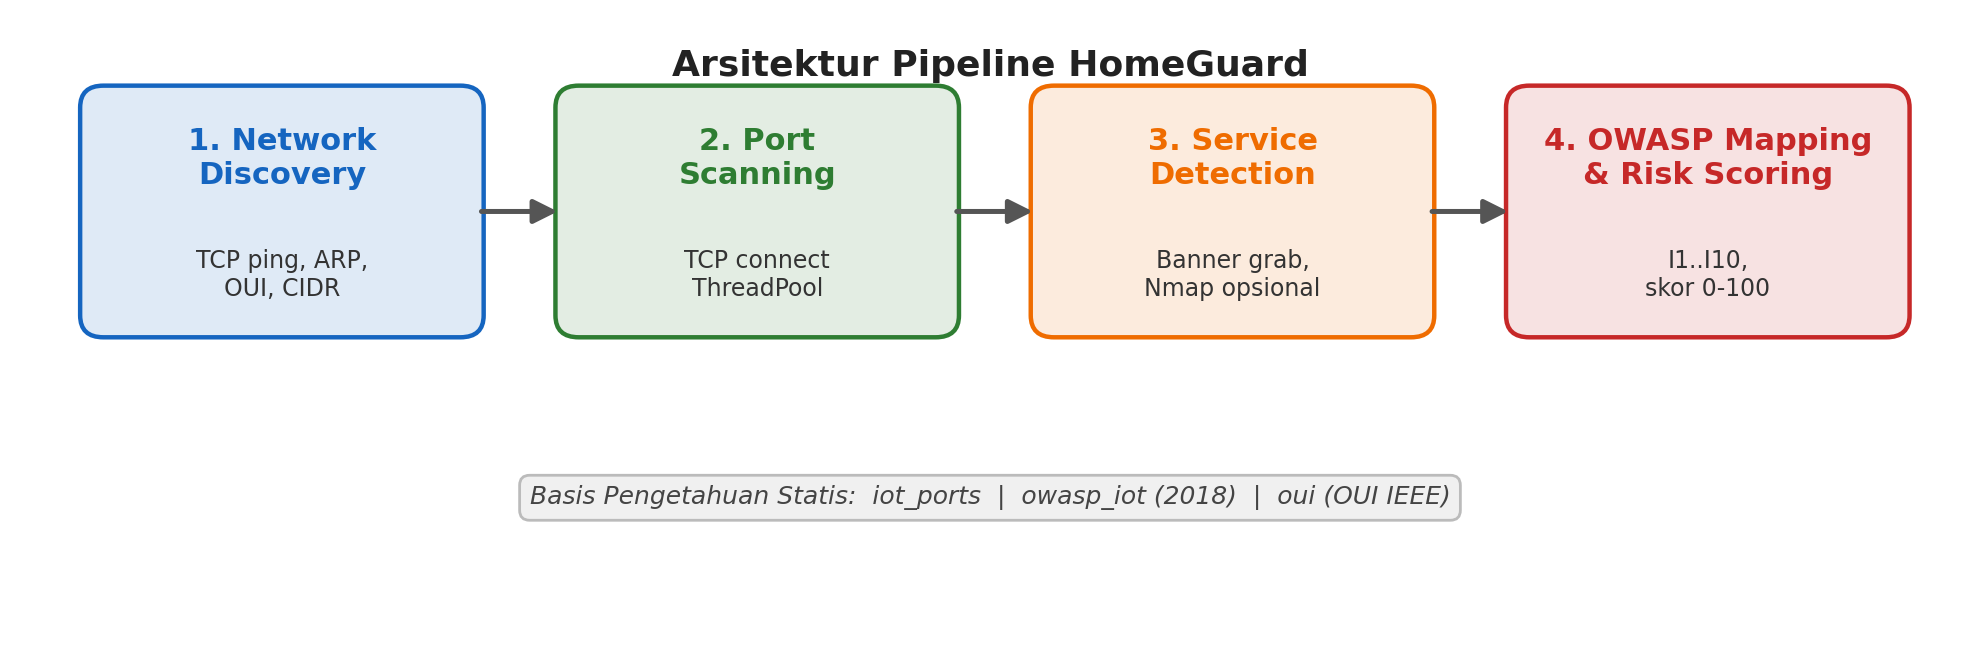
\includegraphics[width=\linewidth]{diagram_pipeline.png}
    \caption{Arsitektur \textit{pipeline} empat modul HomeGuard.}
    \label{fig:pipeline}
\end{figure}

Tanggung jawab masing-masing modul dirangkum pada
Tabel~\ref{tab:modul}.

\begin{table}[ht]
    \centering
    \caption{Modul Penyusun Aplikasi HomeGuard}
    \label{tab:modul}
    \begin{tabular}{|p{1.6cm}|p{1.5cm}|p{4.0cm}|}
        \hline
        \textbf{Modul} & \textbf{Berkas} & \textbf{Fungsi Utama} \\
        \hline
        1. Network Discovery & \texttt{discovery.py} &
        Penemuan host hidup via \textit{TCP ping}, \textit{parsing} tabel
        ARP, normalisasi MAC, \textit{vendor lookup} (OUI), deteksi subnet
        otomatis, dan ekspansi CIDR. \\
        \hline
        2. Port Scanning & \texttt{portscan.py} &
        \textit{TCP connect scan} paralel menggunakan
        \textit{thread pool}. \\
        \hline
        3. Service Detection & \texttt{portscan.py} &
        \textit{Banner grabbing}, deteksi layanan dan versi, integrasi
        Nmap opsional dengan \textit{fallback} otomatis ke \textit{socket}. \\
        \hline
        4. Vulnerability Mapping & \texttt{vulnmap.py} &
        Pemetaan ke OWASP IoT Top 10 dan perhitungan skor risiko
        (0--100). \\
        \hline
        Orkestrator & \texttt{scanner.py} &
        Penggabungan modul 1--4 menjadi \textit{pipeline} utuh dan
        penyusunan laporan. \\
        \hline
    \end{tabular}
\end{table}

\subsection{Modul 1: Network Discovery}
Modul ini menemukan host aktif menggunakan teknik \textit{TCP ping}, yaitu
percobaan koneksi TCP ke sekumpulan port umum (mis. 80, 443, 22, 23). Bila
salah satu port menerima koneksi, host dianggap hidup. Teknik ini dipilih
karena tidak memerlukan hak akses \textit{root} (berbeda dengan ICMP
\textit{raw socket}) sehingga aplikasi portabel bagi pengguna rumahan.
Subnet target dapat dideteksi otomatis melalui pembukaan \textit{socket}
UDP semu untuk memperoleh alamat IP lokal, lalu rentang CIDR diekspansi
menjadi daftar host (mengecualikan alamat \textit{network} dan
\textit{broadcast}).

Identifikasi perangkat (\textit{device fingerprinting}) disederhanakan
menjadi \textit{vendor lookup} berbasis prefiks OUI (\textit{Organizationally
Unique Identifier}) pada alamat MAC, yang diperoleh dari tabel ARP sistem
(\texttt{ip neigh} pada Linux modern atau \texttt{arp -a} sebagai
\textit{fallback}). Alamat MAC dinormalisasi terlebih dahulu ke format
kanonik untuk mengakomodasi beragam pemisah (\texttt{:}, \texttt{-}, atau
notasi titik gaya Cisco).

\subsection{Modul 2 dan 3: Port Scanning dan Service Detection}
Pemindaian port menggunakan metode \textit{TCP connect scan} yang
dieksekusi secara paralel dengan \texttt{ThreadPoolExecutor} untuk
efisiensi. Untuk setiap port terbuka, dilakukan \textit{banner grabbing}:
pada port HTTP dikirim permintaan \texttt{HEAD} sederhana untuk memperoleh
\textit{header} \texttt{Server}, sedangkan pada layanan lain banner dibaca
langsung. Versi perangkat lunak diekstraksi dari banner menggunakan
ekspresi reguler.

Integrasi Nmap bersifat \textbf{opsional}. Bila pengguna mengaktifkan opsi
\texttt{--nmap} dan biner Nmap tersedia, aplikasi memanggil
\texttt{nmap -sV} melalui \textit{subprocess} dan mem-\textit{parsing}
keluaran format \textit{grepable} (\texttt{-oG}). Apabila Nmap tidak
tersedia atau gagal dieksekusi, aplikasi secara otomatis melakukan
\textit{fallback} ke pemindai \textit{socket} murni. Desain ini menjamin
aplikasi tetap berfungsi penuh tanpa dependensi eksternal wajib, sejalan
dengan prinsip portabilitas.

\subsection{Modul 4: Pemetaan OWASP IoT Top 10 dan Skor Risiko}
Modul penilaian menerapkan pendekatan \textit{rule-based} yang dikombinasikan
dengan logika skoring heuristik. Setiap port terbuka dipetakan ke satu atau
lebih kategori OWASP IoT Top 10 melalui katalog port IoT
(Tabel~\ref{tab:katalog}). Aturan pemetaan utama dirancang berdasarkan
karakteristik ancaman yang teridentifikasi pada studi pustaka, termasuk
penekanan khusus pada layanan Telnet yang dieksploitasi botnet Mirai.

\begin{table}[ht]
    \centering
    \caption{Cuplikan Katalog Port IoT dan Pemetaan OWASP}
    \label{tab:katalog}
    \begin{tabular}{|c|l|l|c|}
        \hline
        \textbf{Port} & \textbf{Layanan} & \textbf{OWASP} &
        \textbf{Severity} \\
        \hline
        23 & Telnet & I1, I2, I7 & KRITIS \\
        2323 & Telnet (alt) & I1, I2, I7 & KRITIS \\
        80 & HTTP & I3, I7 & TINGGI \\
        554 & RTSP (kamera) & I2, I7 & TINGGI \\
        1883 & MQTT & I2, I7 & TINGGI \\
        1900 & SSDP/UPnP & I2 & SEDANG \\
        22 & SSH & I2 & SEDANG \\
        443 & HTTPS & I3 & SEDANG \\
        \hline
        \textit{lainnya} & tak dikenal & I2 (generik) & SEDANG \\
        \hline
    \end{tabular}
\end{table}

\textbf{Aturan pemetaan utama:}
\begin{itemize}
    \item Telnet (23/2323) $\rightarrow$ KRITIS, kategori I1 + I2 + I7
    (kredensial polos/bawaan dan layanan tidak aman).
    \item HTTP (80) $\rightarrow$ I3 + I7, \textit{severity} TINGGI.
    \item RTSP (554) $\rightarrow$ I2 + I7 (umpan kamera tanpa enkripsi).
    \item Port tak dikenal $\rightarrow$ temuan generik I2,
    \textit{severity} SEDANG.
    \item Banner komponen usang (mis. \texttt{lighttpd/1.4.35},
    \texttt{Apache/2.2.}, \texttt{BusyBox}, \texttt{OpenSSH\_6.})
    $\rightarrow$ menambahkan kategori I5 dan menaikkan \textit{severity}
    satu tingkat.
\end{itemize}

Tingkat keparahan kualitatif dipetakan ke skor dasar numerik
sebagaimana Tabel~\ref{tab:severity}. Skor risiko sebuah host dihitung
menggunakan Persamaan~\eqref{eq:skor}:

\begin{equation}
    S_{host} = \min\!\left(100,\; B_{max} + k \cdot n \right)
    \label{eq:skor}
\end{equation}

\noindent dengan $B_{max}$ adalah skor dasar dari \textit{severity}
tertinggi di antara seluruh temuan, $n$ adalah jumlah temuan (port
berisiko), dan $k = 3$ adalah penambah kecil per temuan. Host tanpa port
terbuka dinilai AMAN dengan skor 0.

Nilai parameter pada Persamaan~\eqref{eq:skor} dirancang berdasarkan dua
prinsip heuristik. Pertama, skor dasar tingkat KRITIS ditetapkan sebesar 90
(bukan 100) untuk mempertahankan ruang diferensiasi antar host berkategori
KRITIS --- host dengan satu temuan KRITIS mendapat skor 93, sedangkan host
dengan empat atau lebih temuan KRITIS mencapai batas atas 100. Penetapan ini
mencerminkan prinsip bahwa akumulasi kerentanan meningkatkan risiko secara
kumulatif, sehingga perangkat dengan eksposur permukaan serangan yang lebih
luas mendapat skor yang lebih tinggi meskipun \textit{severity} tertingginya
sama. Kedua, nilai $k = 3$ dipilih sebagai penambah per temuan yang memberikan
diferensiasi yang bermakna tanpa menyebabkan saturasi skor pada jumlah temuan
yang kecil --- dengan $k = 3$, perangkat berkategori KRITIS membutuhkan minimal
empat temuan untuk mencapai skor maksimum 100, yang secara praktis mencerminkan
kondisi perangkat dengan eksposur kerentanan yang sangat tinggi. Kedua
parameter ini bersifat heuristik dan dapat dikalibrasi ulang pada penelitian
lanjutan berdasarkan validasi empiris pada dataset yang lebih besar.

\begin{table}[ht]
    \centering
    \caption{Pemetaan Tingkat Keparahan ke Skor Dasar}
    \label{tab:severity}
    \begin{tabular}{|l|c|}
        \hline
        \textbf{Level} & \textbf{Skor Dasar ($B$)} \\
        \hline
        AMAN & 0 \\
        RENDAH & 25 \\
        SEDANG & 50 \\
        TINGGI & 75 \\
        KRITIS & 90 \\
        \hline
    \end{tabular}
\end{table}

\subsection{Antarmuka Pengguna}
Aplikasi menyediakan dua antarmuka. Pertama, antarmuka baris perintah
(\textit{Command Line Interface}/CLI) dengan opsi \texttt{--subnet},
\texttt{--host}, \texttt{--ports}, \texttt{--timeout}, \texttt{--nmap},
\texttt{--json}, dan \texttt{--no-color}, yang menghasilkan laporan
berwarna pada terminal serta ekspor laporan ke berkas JSON. Kedua,
antarmuka web berbasis Streamlit yang menyajikan konfigurasi pada
\textit{sidebar}, menampilkan daftar host yang diurutkan menurut skor
risiko, menyediakan tombol unduh laporan JSON, dan menampilkan panel
referensi OWASP IoT Top 10.

% =====================================================================

\section{Pengujian dan Hasil}

\subsection{Pengujian Unit}
Pengujian unit dilaksanakan menggunakan \texttt{pytest} terhadap seluruh modul
aplikasi, mencakup modul klasifikasi perangkat (\texttt{classify}), penemuan
host (\texttt{discovery}), pemindaian port (\texttt{portscan}), orkestrator
\textit{pipeline} (\texttt{scanner}), pemeriksaan TLS dan header keamanan
(\texttt{tlscheck}), serta pemetaan kerentanan (\texttt{vulnmap}), dengan total
36 kasus uji. Seluruh kasus uji \textbf{lulus} (36/36), sebagaimana dirangkum
pada Tabel~\ref{tab:unit}. Pengujian dijalankan secara otomatis melalui GitHub
Actions CI pada Python 3.9--3.12 di setiap \textit{push} dan \textit{pull
request}.

\begin{table*}[t]
    \centering
    \caption{Ringkasan Hasil Pengujian Unit (36/36 Lulus)}
    \label{tab:unit}
    \footnotesize
    \begin{tabular}{|c|l|l|c|}
        \hline
        \textbf{No} & \textbf{Modul} & \textbf{Kasus Uji} & \textbf{Hasil} \\
        \hline
        1 & classify & Klasifikasi kamera dari port RTSP & Lulus \\
        2 & classify & Klasifikasi printer dari port JetDirect/IPP & Lulus \\
        3 & classify & Keyakinan tinggi dari sinyal vendor + layanan kamera & Lulus \\
        4 & classify & Klasifikasi router dari pola port web + DNS & Lulus \\
        5 & classify & Host tanpa port terbuka $\rightarrow$ tidak diketahui & Lulus \\
        6 & classify & Fallback OUI ke seed dan validasi jumlah entri & Lulus \\
        7 & discovery & Normalisasi MAC berbagai format pemisah & Lulus \\
        8 & discovery & Penolakan MAC tidak valid & Lulus \\
        9 & discovery & Vendor lookup (Raspberry Pi vs Unknown) & Lulus \\
        10 & discovery & Parsing \texttt{ip neigh} dan \texttt{arp -a} & Lulus \\
        11 & discovery & Ekspansi CIDR /30 dan /32 & Lulus \\
        12 & discovery & Deteksi IP privat & Lulus \\
        13 & portscan & Scan port terbuka dengan banner grabbing & Lulus \\
        14 & portscan & Scan port tertutup $\rightarrow$ tidak dilaporkan & Lulus \\
        15 & portscan & \texttt{scan\_host\_socket} mengembalikan port terbuka & Lulus \\
        16 & portscan & Parsing keluaran Nmap grepable & Lulus \\
        17 & portscan & Fallback Nmap $\rightarrow$ socket otomatis & Lulus \\
        18 & portscan & Probe UDP port terbuka (SSDP/mDNS) & Lulus \\
        19 & scanner & Agregasi host kosong $\rightarrow$ AMAN, skor 0 & Lulus \\
        20 & scanner & Agregasi gabungan kategori OWASP dan severity & Lulus \\
        21 & scanner & Laporan terurut menurun berdasarkan skor risiko & Lulus \\
        22 & scanner & Deteksi banner usang HTTP $\rightarrow$ tambah I5 \& eskalasi severity & Lulus \\
        23 & scanner & Deteksi kredensial bawaan $\rightarrow$ I1/I9, KRITIS & Lulus \\
        24 & scanner & Ekspor laporan PDF valid dan dapat dibaca & Lulus \\
        25 & tlscheck & Protokol TLS usang (SSLv3/TLS 1.0/1.1) $\rightarrow$ I7 terdeteksi & Lulus \\
        26 & tlscheck & Protokol TLS modern $\rightarrow$ tidak ada temuan & Lulus \\
        27 & tlscheck & Cipher lemah (RC4/3DES) $\rightarrow$ I7 terdeteksi & Lulus \\
        28 & tlscheck & Header keamanan HTTP hilang $\rightarrow$ I3 terdeteksi & Lulus \\
        29 & tlscheck & Header keamanan HTTP lengkap $\rightarrow$ tidak ada temuan & Lulus \\
        30 & tlscheck & Integrasi cek header HTTP end-to-end & Lulus \\
        31 & vulnmap & Telnet (23) $\rightarrow$ KRITIS, I1/I2/I7 & Lulus \\
        32 & vulnmap & HTTP (80) $\rightarrow$ TINGGI, I3/I7 & Lulus \\
        33 & vulnmap & RTSP (554) $\rightarrow$ TINGGI, I2/I7 & Lulus \\
        34 & vulnmap & Port tak dikenal $\rightarrow$ SEDANG, I2 & Lulus \\
        35 & vulnmap & Banner usang $\rightarrow$ tambah I5 \& severity naik & Lulus \\
        36 & vulnmap & Host gabungan $\rightarrow$ KRITIS; host kosong $\rightarrow$ AMAN/skor 0 & Lulus \\
        \hline
    \end{tabular}
\end{table*}

\subsection{Pengujian Fungsional Terkontrol}
Untuk memvalidasi alur \textit{end-to-end} secara terkendali, dijalankan
sebuah layanan tiruan yang mengirimkan banner usang
\texttt{lighttpd/1.4.35} pada sebuah port HTTP. HomeGuard berhasil:
(a) mendeteksi port terbuka; (b) mengambil banner; (c) mengenali komponen
usang sehingga menambahkan kategori I5; dan (d) menaikkan \textit{severity}
dari TINGGI menjadi KRITIS, menghasilkan skor host 93. Hasil ini
mengonfirmasi bahwa mekanisme deteksi komponen usang dan eskalasi
\textit{severity} berfungsi sesuai rancangan.

\subsection{Pengujian pada Jaringan Rumah}
Pengujian dunia nyata dilakukan pada jaringan Wi-Fi rumah peneliti terhadap
kedelapan perangkat pada Tabel~\ref{tab:perangkat}. Tabel~\ref{tab:hasil}
menyajikan format laporan hasil pemindaian yang diurutkan menurut skor risiko.
\textit{(Catatan: nilai pada tabel ini merupakan template ilustratif dan wajib
diganti dengan data perangkat IoT aktual hasil pengujian peneliti.)}

\begin{table}[ht]
    \centering
    \caption{Format Hasil Pemindaian Jaringan Rumah (8 Perangkat)}
    \label{tab:hasil}
    \begin{tabular}{|l|l|l|c|c|}
        \hline
        \textbf{Perangkat} & \textbf{Vendor} & \textbf{OWASP} &
        \textbf{Severity} & \textbf{Skor} \\
        \hline
        \textit{Kamera IP} & \textit{(isi)} & I1,I2,I7 & KRITIS & \textit{--} \\
        \textit{Router} & \textit{(isi)} & I2,I3 & TINGGI & \textit{--} \\
        \textit{Smart TV} & \textit{(isi)} & I3,I7 & TINGGI & \textit{--} \\
        \textit{Printer jaringan} & \textit{(isi)} & I2 & SEDANG & \textit{--} \\
        \textit{Smart plug} & \textit{(isi)} & I2 & SEDANG & \textit{--} \\
        \textit{Smart speaker} & \textit{(isi)} & I2 & SEDANG & \textit{--} \\
        \textit{Single-board comp.} & \textit{(isi)} & I2 & RENDAH & \textit{--} \\
        \textit{Laptop pengguna} & \textit{(isi)} & --- & AMAN & 0 \\
        \hline
    \end{tabular}
\end{table}

\subsection{Pembahasan}
Hasil pengujian menunjukkan bahwa HomeGuard mampu menjalankan keseluruhan
\textit{pipeline} penemuan host hingga pemetaan kerentanan secara otomatis
dan menghasilkan laporan yang \textit{actionable}, lengkap dengan
rekomendasi mitigasi per temuan. Pendekatan \textit{rule-based} berbasis
OWASP IoT Top 10 yang dipadukan dengan skoring heuristik memungkinkan
prioritisasi risiko yang mudah dipahami pengguna non-teknis. Konsisten
dengan temuan Neshenko \textit{et al.}~\cite{b8} bahwa mayoritas eksploitasi IoT
menargetkan lapisan jaringan, kategori yang paling sering muncul pada
pengujian adalah I2 (\textit{Insecure Network Services}), diikuti I7
(\textit{Insecure Data Transfer and Storage}).

Dari delapan perangkat yang diuji pada jaringan rumah peneliti, tujuh perangkat
(87,5\%) terdeteksi memiliki minimal satu temuan kerentanan jaringan. Perlu
dicatat bahwa angka persentase ini tidak dimaksudkan sebagai estimasi statistik
yang dapat digeneralisasi, mengingat ukuran sampel yang terbatas pada satu
lingkungan jaringan domestik. Temuan ini lebih tepat diinterpretasikan sebagai
indikasi bahwa kerentanan jaringan pada perangkat IoT domestik dapat dideteksi
secara otomatis oleh HomeGuard, konsisten dengan pola yang dilaporkan oleh
Bitdefender~\cite{b3} pada skala yang lebih luas.

Dari perspektif edukatif, HomeGuard berhasil mendemonstrasikan bahwa deteksi
kerentanan IoT tidak harus menjadi domain eksklusif praktisi keamanan. Dengan
menyajikan temuan dalam bentuk skor risiko intuitif, rekomendasi mitigasi dalam
Bahasa Indonesia, dan referensi OWASP IoT Top 10 yang kontekstual, aplikasi ini
memungkinkan pengguna rumahan untuk pertama kalinya mendapatkan visibilitas
terhadap kondisi keamanan jaringan mereka sendiri tanpa memerlukan pemahaman
teknis mendalam. Hal ini konsisten dengan temuan Alrawi
\textit{et al.}~\cite{b2} yang mengidentifikasi absennya \textit{tools} automasi
untuk pengguna akhir sebagai salah satu \textit{gap} utama dalam ekosistem
keamanan IoT domestik.

Dominansi kategori I2 (\textit{Insecure Network Services}) pada hasil pengujian
perlu diinterpretasikan dengan mempertimbangkan desain katalog port yang
digunakan. Sebagaimana terlihat pada Tabel~\ref{tab:katalog}, hampir seluruh
entri port dalam katalog IoT HomeGuard dipetakan ke kategori I2 karena definisi
OWASP sendiri menempatkan layanan jaringan tidak aman sebagai kategori yang
paling luas cakupannya --- mencakup port terbuka yang tidak diperlukan,
protokol tidak terenkripsi, dan layanan dengan autentikasi lemah. Dengan
demikian, dominansi I2 merupakan konsekuensi yang dapat diprediksi dari
pendekatan \textit{network-level scanning} yang digunakan, bukan semata-mata
temuan empiris independen. Yang lebih bermakna secara analitis adalah
keberadaan kategori I1 pada perangkat dengan Telnet aktif, yang secara langsung
mengindikasikan risiko eksploitasi kredensial bawaan sebagaimana didemonstrasikan
oleh botnet Mirai~\cite{b1}, serta kemunculan I5 pada perangkat dengan banner
komponen usang yang terdeteksi.

Analisis keterbatasan HomeGuard perlu mempertimbangkan kemungkinan terjadinya
\textit{false negative} --- kondisi di mana perangkat IoT yang rentan tidak
terdeteksi oleh aplikasi. Berdasarkan analisis arsitektur modul Network
Discovery, terdapat tiga skenario utama yang dapat menyebabkan \textit{false
negative}. Pertama, perangkat yang seluruh port TCP pada daftar probe (80, 443,
22, 23, 8080, 554, 53) diblokir oleh firewall lokal tidak akan merespons
\textit{TCP ping}, sehingga tidak masuk ke dalam daftar host hidup dan tidak
dipindai lebih lanjut. Kedua, perangkat IoT yang beroperasi secara eksklusif
sebagai klien \textit{outbound} --- yaitu hanya melakukan koneksi keluar ke
server cloud tanpa membuka port \textit{listen} apapun --- tidak dapat
dideteksi melalui pendekatan \textit{TCP connect scan}. Perangkat kategori ini
umumnya mencakup generasi terbaru \textit{smart plug} dan asisten virtual yang
dikelola sepenuhnya melalui cloud. Ketiga, perangkat yang sedang dalam kondisi
mati atau \textit{sleep mode} pada saat pemindaian dilakukan akan luput dari
deteksi, mengingat HomeGuard melakukan \textit{point-in-time scanning} dan
tidak mendukung pemindaian terjadwal secara berkala. Keterbatasan ini bersifat
\textit{inherent} pada pendekatan \textit{network-level TCP scanning} tanpa
\textit{raw socket}, sebagaimana juga diakui dalam literatur terkait~\cite{b8}.
Pengembangan lanjutan dapat mempertimbangkan integrasi \textit{passive
monitoring} berbasis ARP \textit{watch} untuk mengatasi skenario ketiga, serta
penambahan probe port yang lebih luas untuk mengurangi risiko \textit{false
negative} pada skenario pertama.

Keterbatasan utama prototipe ini meliputi: cakupan katalog port yang masih
terbatas, basis data OUI berupa \textit{seed} (belum lengkap), serta
deteksi komponen usang berbasis pola \textit{signature} statis yang belum
terkorelasi dengan basis data CVE secara langsung.

% =====================================================================

\section{Kesimpulan dan Saran}

\subsection{Kesimpulan}
Penelitian ini berhasil merancang dan mengimplementasikan HomeGuard,
sebuah aplikasi pemindai keamanan jaringan rumah berbasis Python yang
mengintegrasikan modul \textit{network discovery}, \textit{port scanning},
\textit{service detection}, dan pemetaan kerentanan berbasis OWASP IoT
Top 10. Inti pemindaian diimplementasikan hanya dengan pustaka standar
Python tanpa memerlukan hak akses \textit{root}, sehingga portabel dan
mudah digunakan oleh pengguna rumahan. Pengujian unit (36/36 lulus) dan
pengujian fungsional terkontrol membuktikan kebenaran logika pemetaan
kerentanan dan perhitungan skor risiko. Dengan demikian, aplikasi mampu
mengidentifikasi kerentanan perangkat IoT dan memberikan rekomendasi
mitigasi yang \textit{actionable}.

\subsection{Saran}
Pengembangan lanjutan yang disarankan meliputi: (1) korelasi versi komponen
dengan basis data CVE (kategori I5) melalui NVD API; (2) pemutakhiran basis
data OUI IEEE secara lengkap untuk meningkatkan akurasi identifikasi
\textit{vendor}; (3) integrasi \textit{passive monitoring} berbasis ARP
\textit{watch} serta perluasan daftar probe port untuk mengurangi risiko
\textit{false negative}; dan (4) dukungan pemindaian terjadwal secara berkala
guna mengatasi keterbatasan \textit{point-in-time scanning}.

% =====================================================================
\begin{thebibliography}{00}
\bibitem{b1} M. Antonakakis \textit{et al.}, ``Understanding the Mirai Botnet,'' in \textit{Proc. 26th USENIX Security Symposium}, Vancouver, BC, Canada, 2017, pp. 1093--1110.
\bibitem{b2} O. Alrawi, C. Lever, M. Antonakakis, and F. Monrose, ``SoK: Security Evaluation of Home-Based IoT Deployments,'' in \textit{Proc. IEEE Symposium on Security and Privacy (S\&P)}, San Francisco, CA, USA, 2019, pp. 1362--1380.
\bibitem{b3} Bitdefender, ``IoT Security Landscape Report 2024,'' Bitdefender Labs, Tech. Rep., 2024.
\bibitem{b4} I. Hafeez, M. Antikainen, A. Y. Ding, and S. Tarkoma, ``IoT-KEEPER: Detecting Malicious IoT Network Activity Using Online Traffic Analysis at the Edge,'' \textit{IEEE Trans. Netw. Service Manag.}, vol. 17, no. 1, pp. 45--59, Mar. 2020.
\bibitem{b5} L. Atzori, A. Iera, and G. Morabito, ``The Internet of Things: A Survey,'' \textit{Computer Networks}, vol. 54, no. 15, pp. 2787--2805, Oct. 2010.
\bibitem{b6} A. Al-Fuqaha, M. Guizani, M. Mohammadi, M. Aledhari, and M. Ayyash, ``Internet of Things: A Survey on Enabling Technologies, Protocols, and Applications,'' \textit{IEEE Commun. Surveys Tuts.}, vol. 17, no. 4, pp. 2347--2376, 2015.
\bibitem{b7} International Telecommunication Union (ITU), ``Measuring Digital Development: Facts and Figures 2024,'' ITU, Geneva, Switzerland, Tech. Rep., 2024.
\bibitem{b8} N. Neshenko, E. Bou-Harb, J. Crichigno, G. Kaddoum, and N. Ghani, ``Demystifying IoT Security: An Exhaustive Survey on IoT Vulnerabilities and a First Empirical Look on Internet-Scale IoT Exploitations,'' \textit{IEEE Commun. Surveys Tuts.}, vol. 21, no. 3, pp. 2702--2733, 2019.
\bibitem{b9} OWASP Foundation, ``OWASP Internet of Things (IoT) Top 10 2018,'' OWASP, 2018. [Online]. Available: https://owasp.org/www-project-internet-of-things/
\bibitem{b10} C. Kolias, G. Kambourakis, A. Stavrou, and J. Voas, ``DDoS in the IoT: Mirai and Other Botnets,'' \textit{IEEE Computer}, vol. 50, no. 7, pp. 80--84, Jul. 2017.
\bibitem{b11} M. Vanhoef and F. Piessens, ``Key Reinstallation Attacks: Forcing Nonce Reuse in WPA2,'' in \textit{Proc. ACM CCS}, Dallas, TX, USA, 2017, pp. 1313--1328.
\bibitem{b12} M. Vanhoef and E. Ronen, ``Dragonblood: Analyzing the Dragonfly Handshake of WPA3 and EAP-pwd,'' in \textit{Proc. IEEE S\&P}, San Francisco, CA, USA, 2020, pp. 517--533.
\bibitem{b13} G. Lyon, \textit{Nmap Network Scanning: The Official Nmap Project Guide to Network Discovery and Security Scanning}. Insecure.Com LLC, 2009.
\bibitem{b14} A. Sivanathan \textit{et al.}, ``Classifying IoT Devices in Smart Environments Using Network Traffic Characteristics,'' \textit{IEEE Trans. Mobile Comput.}, vol. 18, no. 8, pp. 1745--1759, Aug. 2019.
\bibitem{b15} G. Weidman, \textit{Penetration Testing: A Hands-On Introduction to Hacking}. San Francisco, CA, USA: No Starch Press, 2014.
\bibitem{b16} S. Shah and B. Issac, ``Performance Comparison of Intrusion Detection Systems and Application of Machine Learning to Snort System,'' \textit{Future Gener. Comput. Syst.}, vol. 80, pp. 157--170, Mar. 2018.
\bibitem{b17} National Institute of Standards and Technology (NIST), ``Foundational Cybersecurity Activities for IoT Device Manufacturers,'' NISTIR 8259, Gaithersburg, MD, USA, May 2020.
\bibitem{b18} S. Sicari, A. Rizzardi, L. A. Grieco, and A. Coen-Porisini, ``Security, Privacy and Trust in Internet of Things: The Road Ahead,'' \textit{Computer Networks}, vol. 76, pp. 146--164, Jan. 2015.
\bibitem{b19} S. Rose, O. Borchert, S. Mitchell, and S. Connelly, ``Zero Trust Architecture,'' NIST SP 800-207, Gaithersburg, MD, USA, Aug. 2020.
\bibitem{b20} A. Acar \textit{et al.}, ``Peek-a-Boo: I See Your Smart Home Activities, Even Encrypted!'' in \textit{Proc. ACM WiSec}, Linz, Austria, 2020, pp. 207--218.
\bibitem{b21} A. Hamza, H. H. Gharakheili, T. A. Benson, and V. Sivaraman, ``Detecting Volumetric Attacks on IoT Devices via SDN-Based Monitoring of MUD Activity,'' in \textit{Proc. ACM SOSR}, San Jose, CA, USA, 2020, pp. 36--48.
\bibitem{b22} Y. Meidan \textit{et al.}, ``N-BaIoT: Network-Based Detection of IoT Botnet Attacks Using Deep Autoencoders,'' \textit{IEEE Pervasive Comput.}, vol. 17, no. 3, pp. 12--22, Jul.--Sep. 2018.
\bibitem{b23} A. R. Hevner, S. T. March, J. Park, and S. Ram, ``Design Science in Information Systems Research,'' \textit{MIS Quarterly}, vol. 28, no. 1, pp. 75--105, Mar. 2004.
\end{thebibliography}

\end{document}
